%%%% Header %%%%%%%%%%%%%%%%%%%%%%%%%%%%%%%%%%%%%%%%%%%%%%%%%%%%%%%%%%%%%%%%%%%

\documentclass{beamer}

%%%% Packages %%%%%%%%%%%%%%%%%%%%%%%%%%%%%%%%%%%%%%%%%%%%%%%%%%%%%%%%%%%%%%%%%

% font/encoding
\usepackage[utf8]{inputenc} % .tex-file text encoding
\usepackage[T1]{fontenc} % vector fonts and hiQual special chars in output
\usepackage{libertine} % libertine font family
\usepackage[libertine]{newtxmath} % libertine mathematics
\usepackage[scaled=0.85]{inconsolata} % monospace font

% localization
\usepackage[english]{babel} % document language/localization

% maths
\usepackage{amsmath} % various maths features
\usepackage{mathtools} % aligned matrices

% figures
\usepackage{graphicx} % include external images
\usepackage[compatibility=false]{caption}
\usepackage{subcaption} % captions for subfigures

% tables
\usepackage{booktabs} % nice table rules
\usepackage{dcolumn} % column alignment at decimal point

% bibliography
\usepackage[style = authoryear-ibid, % bibliography using biblatex
            backend = biber,
            bibencoding = utf8,
            doi = false,
            isbn = false]{biblatex}

%%%% General layout %%%%%%%%%%%%%%%%%%%%%%%%%%%%%%%%%%%%%%%%%%%%%%%%%%%%%%%%%%%

\usetheme{default} % minimal theme
\usecolortheme{dove}
% \useinnertheme{default}
% \useoutertheme[subsection=false,
%                footline=empty]{miniframes} % cool progress bar
\setbeamertemplate{navigation symbols}{} % no nav symbols
\setbeamertemplate{footline}[page number]
\setbeamertemplate{itemize items}[triangle]
\setbeamertemplate{bibliography item}{} % no bibliography icon
\setkeys{Gin}{width=1.0\textwidth} % figures fill textwidth
% no caption label
\setbeamertemplate{caption}{\insertcaption}
\setbeamertemplate{caption label separator}{}
\hypersetup{pdfstartview={Fit}} % fits the presentation to the window
\usefonttheme{serif}
\setbeamerfont{frametitle}{series=\bfseries}

%%%% Special layout %%%%%%%%%%%%%%%%%%%%%%%%%%%%%%%%%%%%%%%%%%%%%%%%%%%%%%%%%%%

% figure placeholder (comment out to diable)
% \makeatletter
%   \AtBeginDocument{%
%     \def\Ginclude@graphics#1{%
%       \begingroup\fboxsep=-\fboxrule
%       \fbox{\rule{\@ifundefined{Gin@@ewidth}{150pt}{\Gin@@ewidth}}{0pt}%
%         \rule{0pt}{\@ifundefined{Gin@@eheight}{100pt}{\Gin@@eheight}}}\endgroup}}
% \makeatother

%%%% Tables %%%%%%%%%%%%%%%%%%%%%%%%%%%%%%%%%%%%%%%%%%%%%%%%%%%%%%%%%%%%%%%%%%%

% global table format
\newcommand{\tabformat}{\small\centering}
% fontsize of table footnote
\newcommand{\tabfontsizefoot}{\footnotesize}
% dcolumn column type
\newcolumntype{d}{D{,}{,}}
% centering with fixed column size in tables
\newcolumntype{Q}[1]{>{\centering\arraybackslash}p{#1}}
% raggedright in tables
\newcolumntype{P}[1]{>{\raggedright\hspace{0pt}\arraybackslash}p{#1}}
% no space between table columns
\renewcommand{\tabcolsep}{0cm}

%%%% Paths %%%%%%%%%%%%%%%%%%%%%%%%%%%%%%%%%%%%%%%%%%%%%%%%%%%%%%%%%%%%%%%%%%%%

% figures
\graphicspath{{/home/jon/lucile/share/hive/sci/viscomplexis/fig/}}

% bibliography file
\bibliography{/home/jon/lucile/share/hive/sci/refs/refs.bib}

%%%% meta data %%%%%%%%%%%%%%%%%%%%%%%%%%%%%%%%%%%%%%%%%%%%%%%%%%%%%%%%%%%%%%%%

\title{Visualizing Composite Data on the Lexis Surface}
\subtitle{What share of a population features\\attribute $i$ at period $t$ and age $x$?}
\author{Jonas Schöley\\\url{schoeley@demogr.mpg.de}}
\institute{
\includegraphics[width = 3cm]{./misc/EDSDLogo.pdf}}
\subject{Visualizing composite data on the Lexis surface}
\keywords{data visualization, compositional data, Lexis surface, causes of death}

%%%% titlepage %%%%%%%%%%%%%%%%%%%%%%%%%%%%%%%%%%%%%%%%%%%%%%%%%%%%%%%%%%%%%%%%

\setbeamerfont{title}{size=\LARGE, series=\bfseries}
\setbeamerfont{subtitle}{size=\Large, series=\mdseries}
\setbeamerfont{author}{size = \normalsize, series=\mdseries}
\setbeamerfont{institute}{size=\normalsize, series=\mdseries}
\defbeamertemplate*{title page}{customized}[1][]
{
  \centering
  \usebeamerfont{title}\inserttitle\\\medskip
  \usebeamerfont{subtitle}\usebeamercolor[fg]{subtitle}\insertsubtitle\par
  \vfill
  \usebeamerfont{author}\insertauthor\par
  \vfill
  \usebeamerfont{institute}\insertinstitute\par
  \usebeamercolor[fg]{titlegraphic}\inserttitlegraphic
}

\begin{document}

{
\usebackgroundtemplate{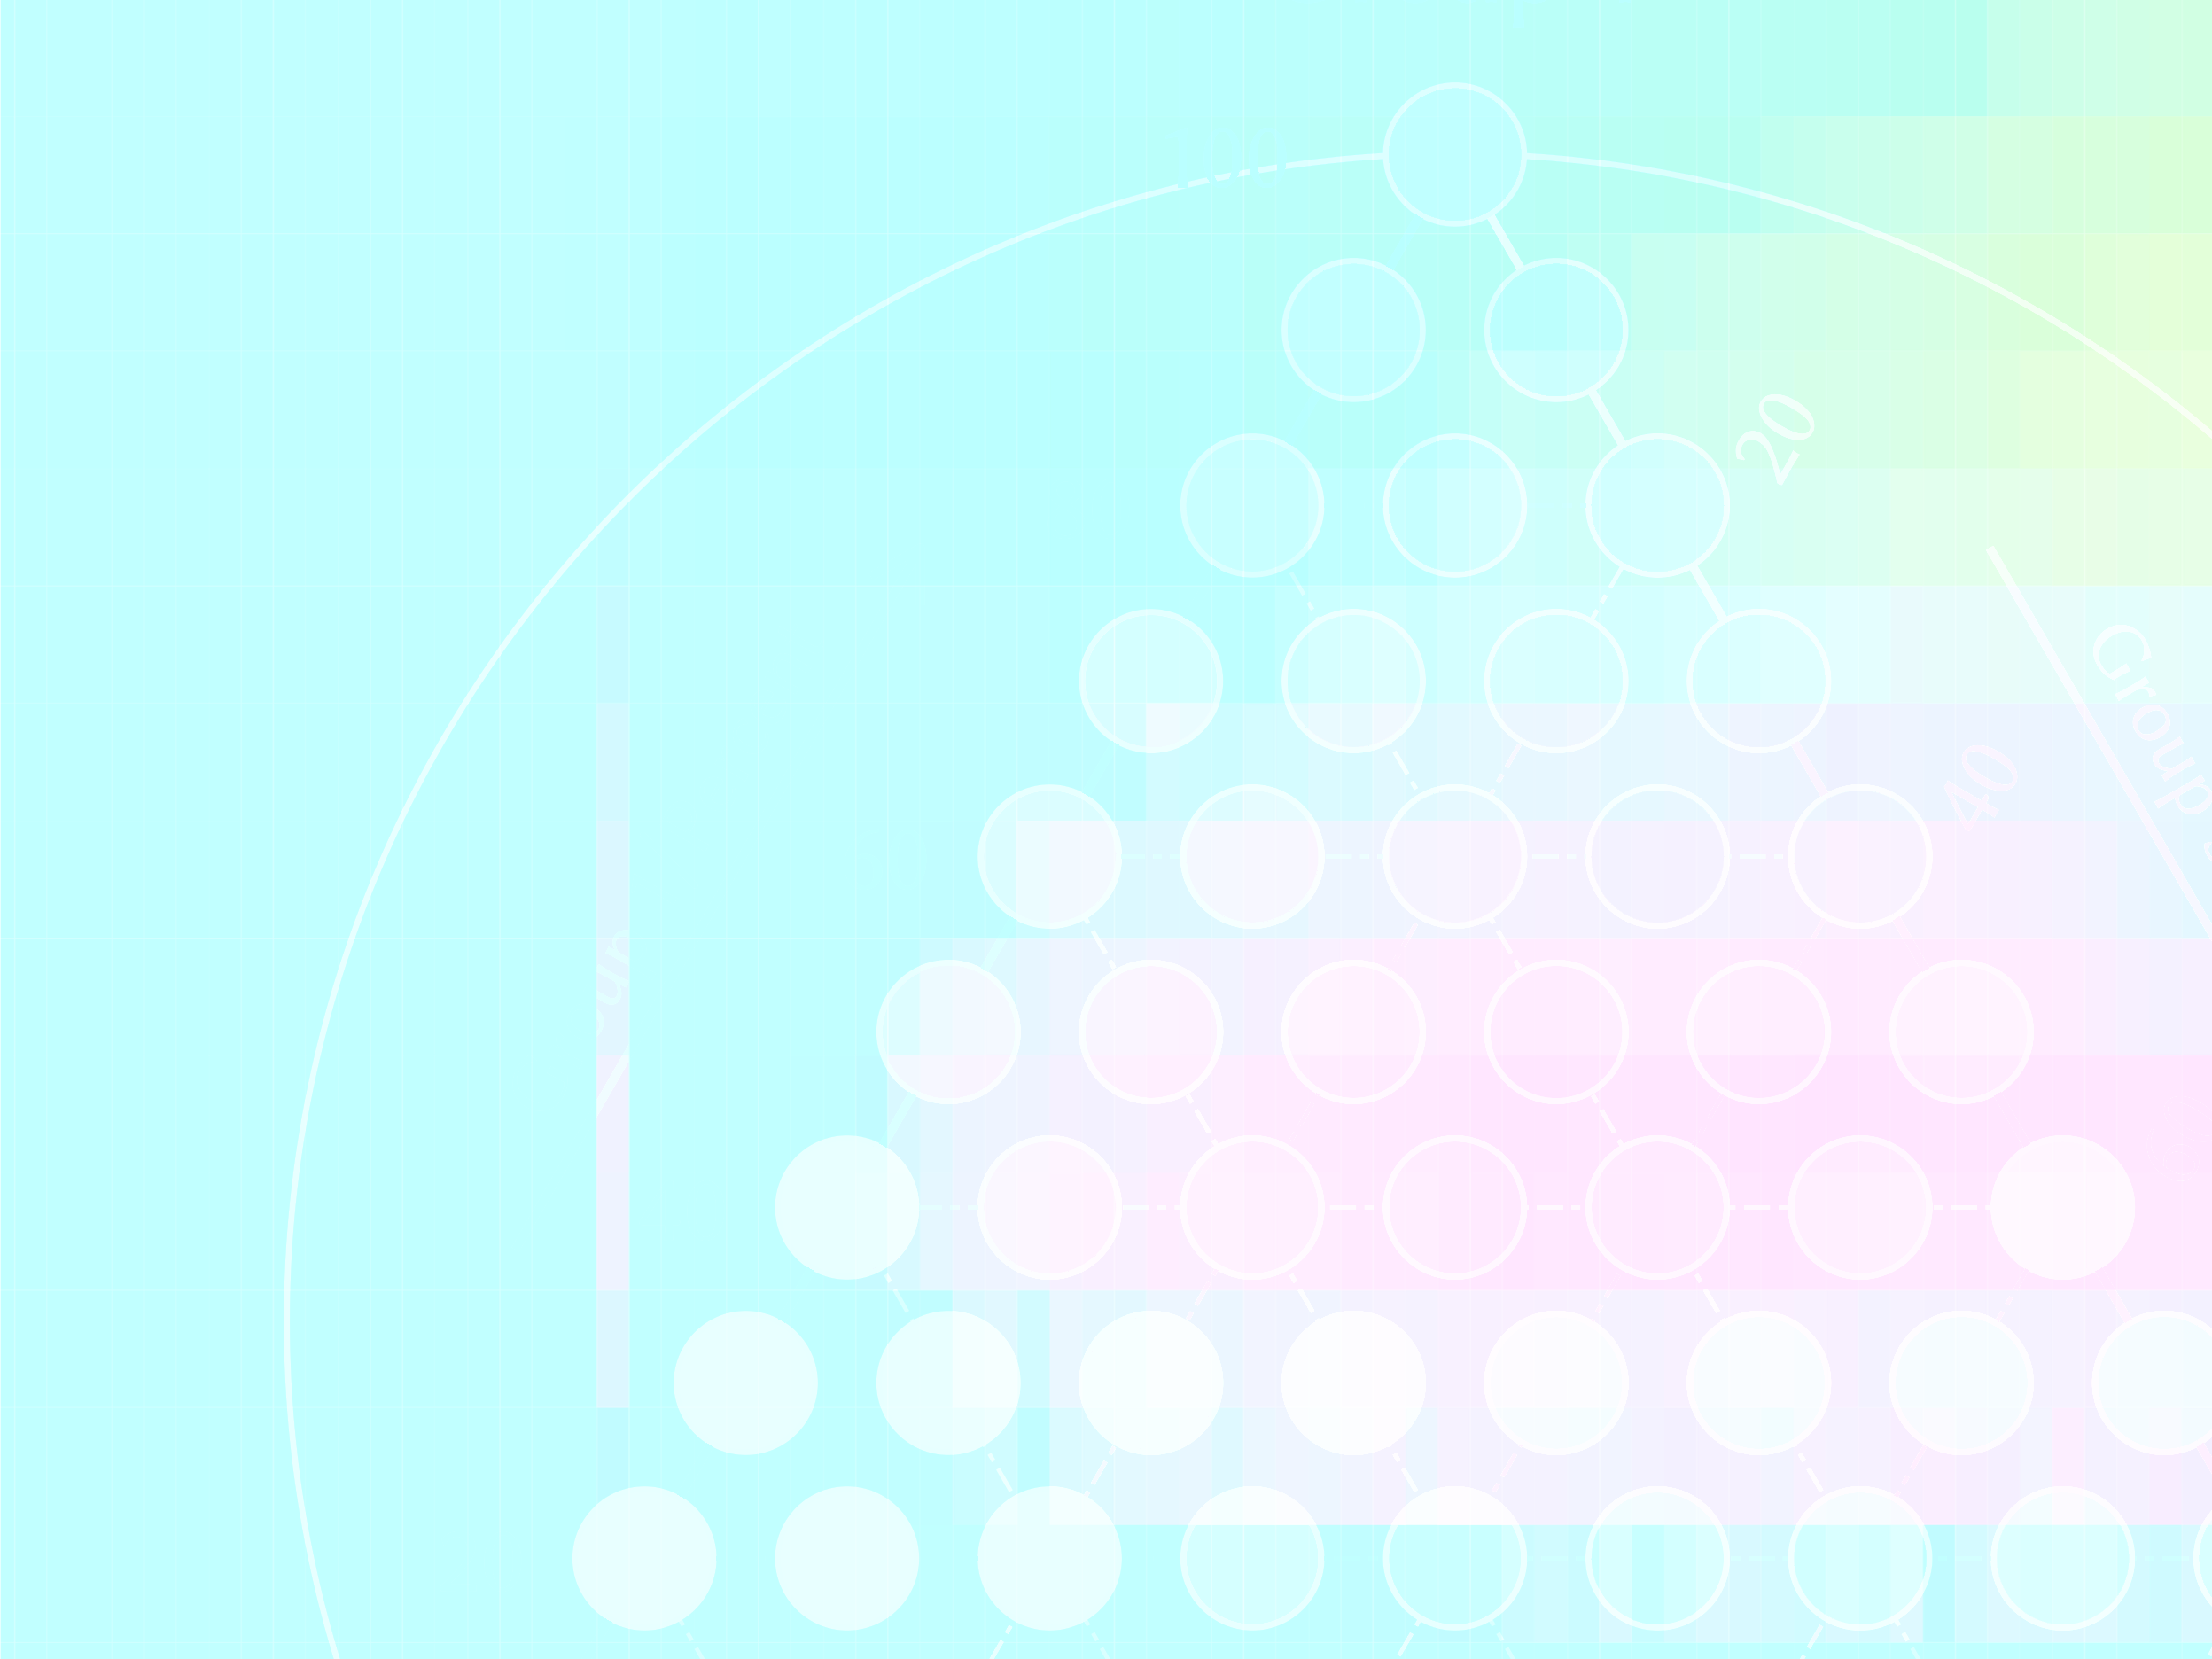
\includegraphics[width=\paperwidth]{./misc/background.png}}%
\begin{frame}[plain]
\titlepage
\end{frame}
}

\section{Predefined Visual Spaces} %%%%%%%%%%%%%%%%%%%%%%%%%%%%%%%%%%%%%%%%%%%%

%\usebackgroundtemplate{\includegraphics[width=\paperwidth]{./misc/background2.png}}

\begin{frame}{pause}
\frametitle{\insertsection}

\begin{columns}[c]

\column{0.73\textwidth}
\begin{figure}[!htb]
\centering
\begin{subfigure}[c]{\textwidth}
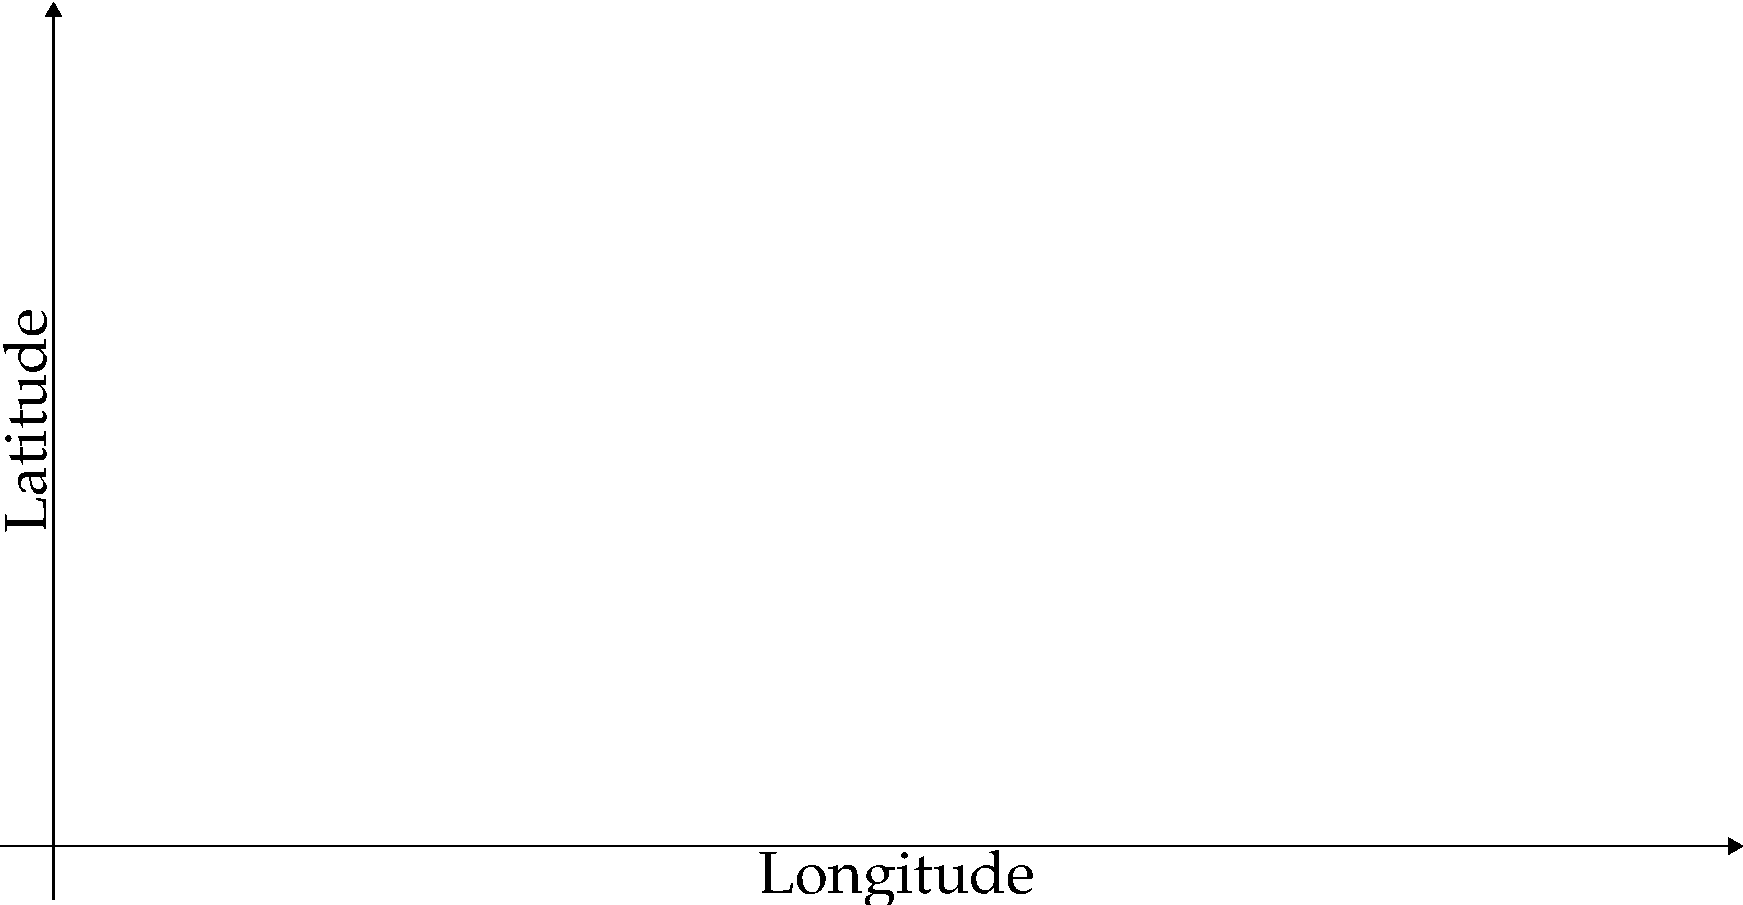
\includegraphics[width = \textwidth]{../fig/plot-spatial_map_empty.pdf}
\end{subfigure}\\
\begin{subfigure}[c]{\textwidth}
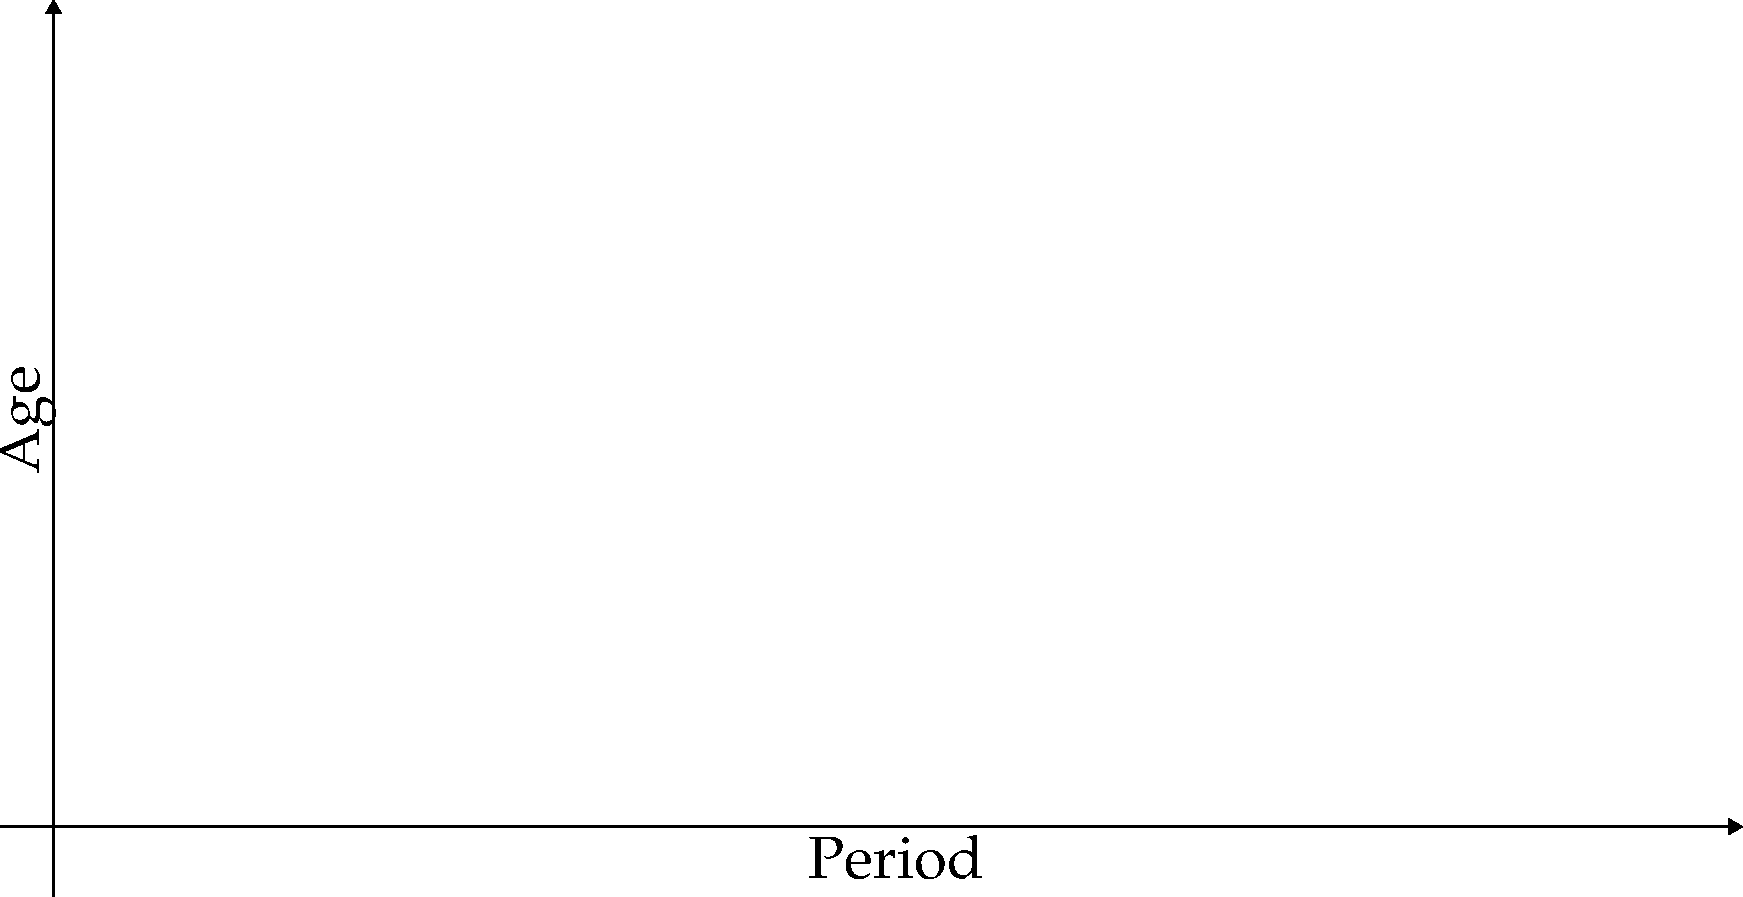
\includegraphics[width = \textwidth]{../fig/plot-temporal_map_empty.pdf}
\end{subfigure}
\end{figure}

\column{0.27\textwidth}
\footnotesize\textbf{A spatial map}.

\vspace{2.5cm}

\footnotesize\textbf{A temporal map}.

\end{columns}

\end{frame}

%

\begin{frame}{pause}
\frametitle{\insertsection}

\begin{columns}[c]

\column{0.73\textwidth}
\begin{figure}[!htb]
\centering
\begin{subfigure}[c]{\textwidth}
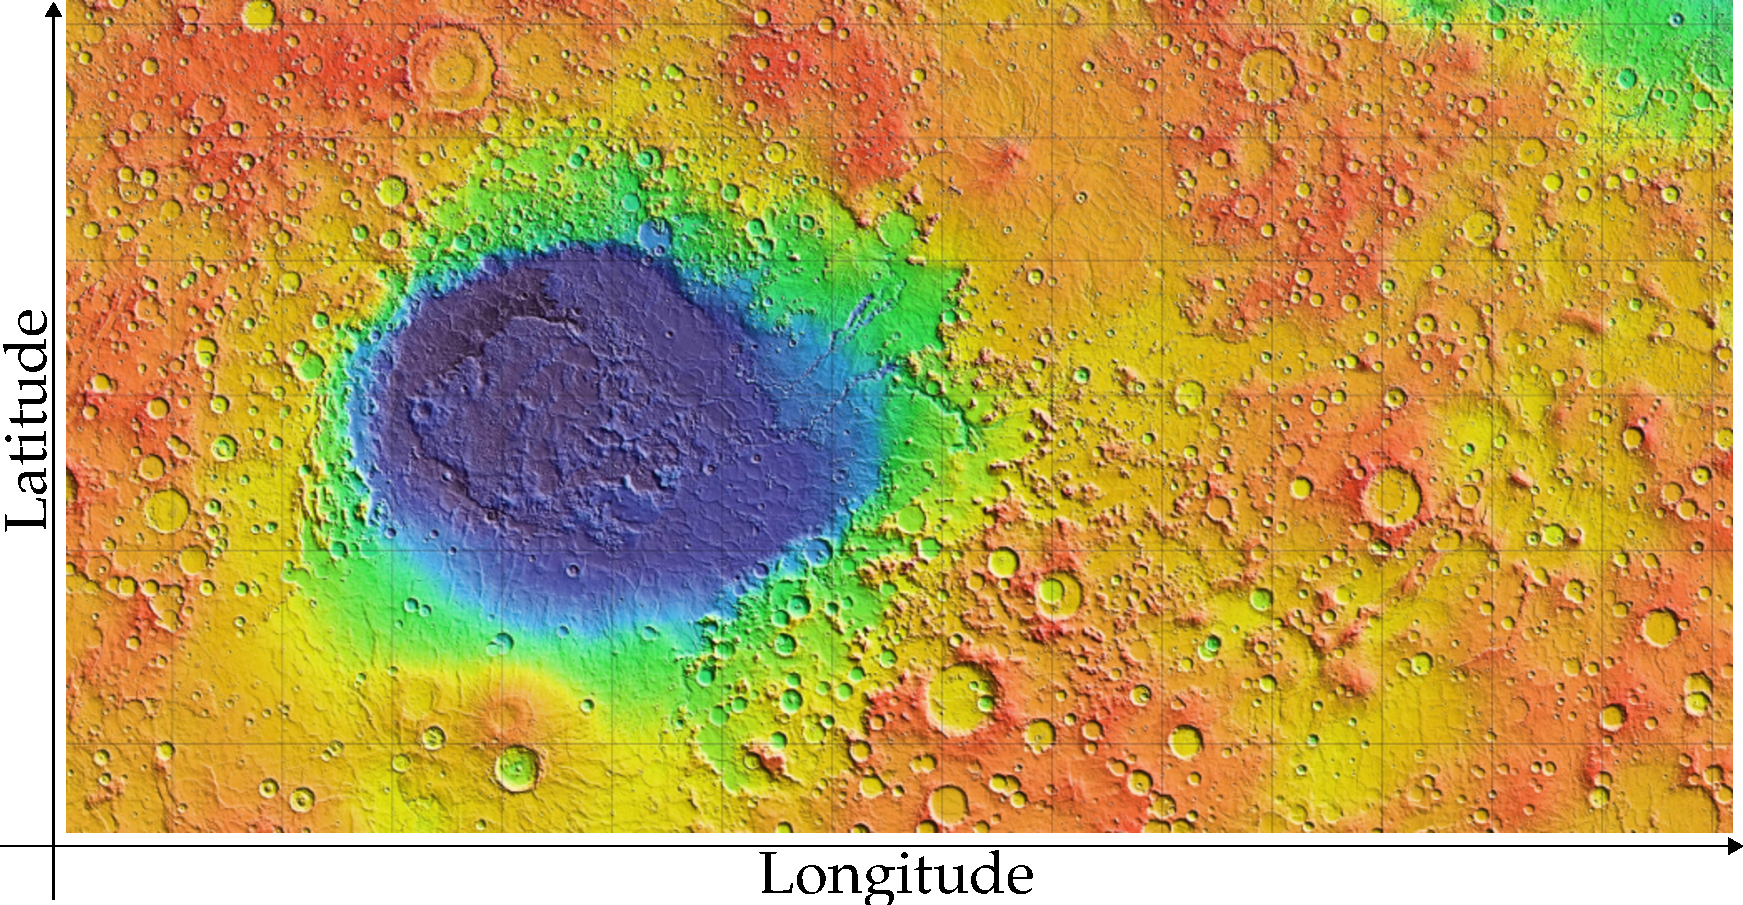
\includegraphics[width = \textwidth]{../fig/plot-spatial_map.pdf}
\end{subfigure}\\
\begin{subfigure}[c]{\textwidth}
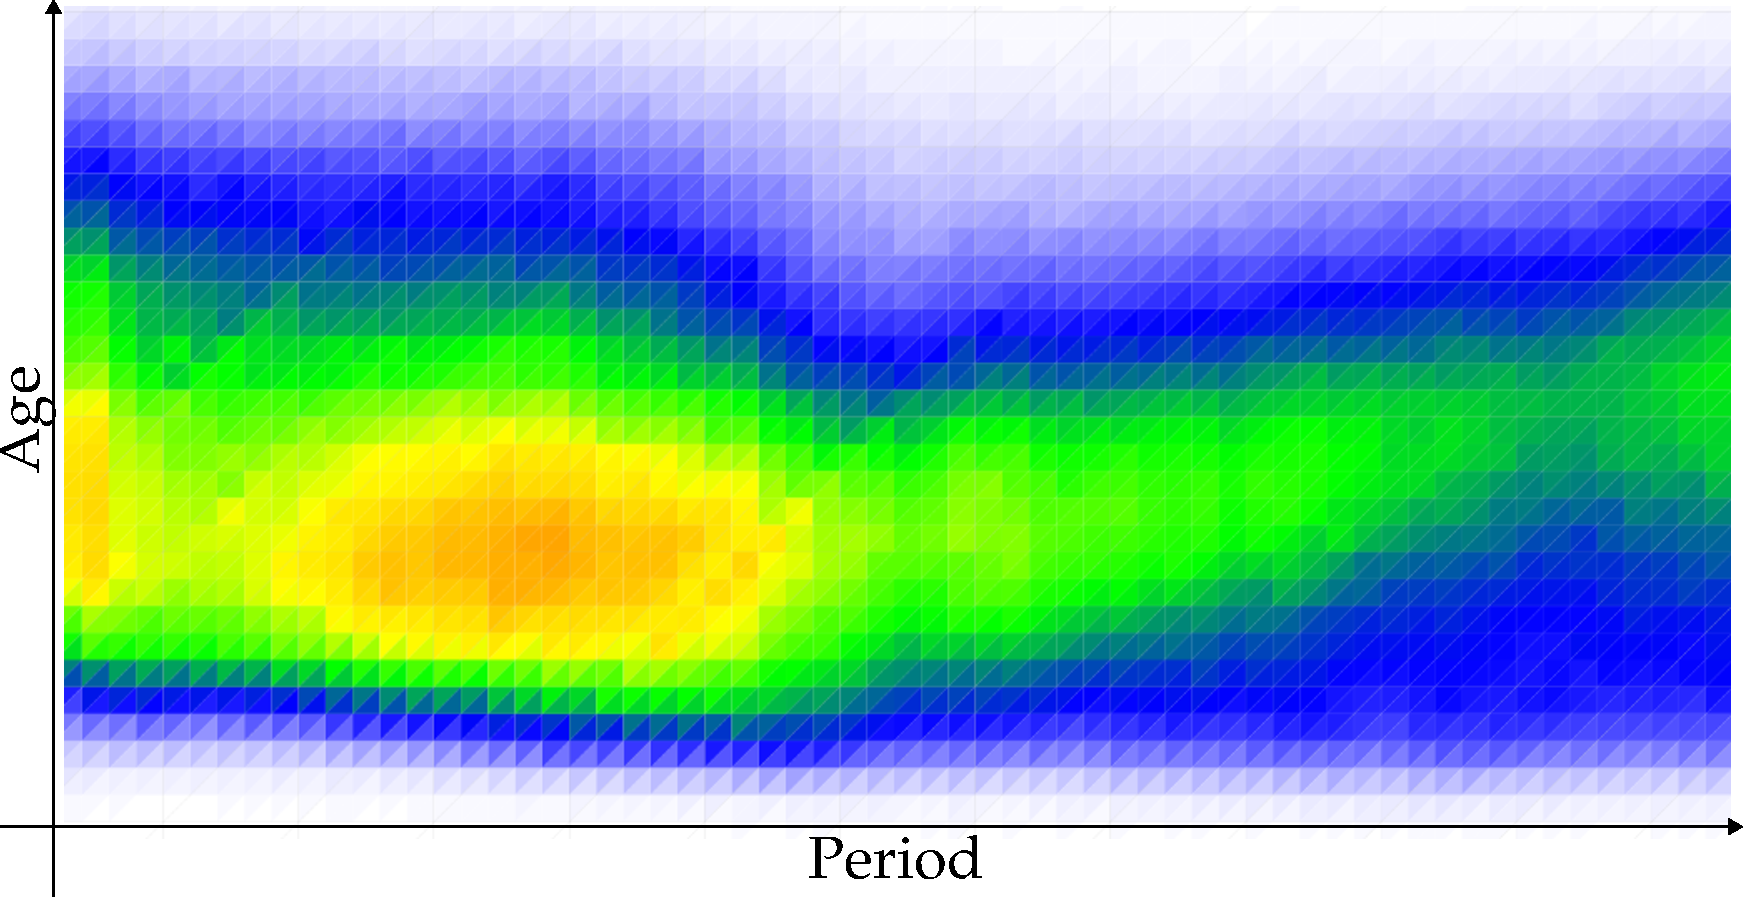
\includegraphics[width = \textwidth]{../fig/plot-temporal_map.pdf}
\end{subfigure}
\end{figure}

\column{0.27\textwidth}
\footnotesize\textbf{A spatial map}\\ The surface of Mars with elevation encoded by colour. \scriptsize\emph{NASA 2000}.

\vspace{2.5cm}

\footnotesize\textbf{A temporal map}\\ Fertility rates in Scotland since 1945 with rate encoded by colour. \scriptsize\emph{Modified from \cite{Riffe2011}.}

\end{columns}

\end{frame}

\section{Plotting Data: Magnitudes vs.~Compositions} %%%%%%%%%%%%%%%%%%%%%%%%%%

\begin{frame}
\frametitle{\insertsection}

$$
\begin{matrix*}[c]
\mbox{\Large$\mathit{Easy}$} & & \mbox{\Large$\mathfrak{Hard}$} \\\midrule
187 \dfrac {\text{Deaths}} {10\,000~\text{Persons}} &
\Longleftarrow &
\begin{pmatrix*}[l]
93 & \text{Neoplasm} \\
40 & \text{Cardiovascular} \\
23 & \text{Respiratory} \\
12 & \text{Accident} \\
19 & \text{Other}
\end{pmatrix*} \\
\text{Single~value} & \text{composed~of} & \text{n-dimensional~vector} \\
& & & \\
& & \Downarrow \text{expressed~as} \\
& & & \\
& & \begin{pmatrix*}[l]
0.50 & \text{Neoplasm} \\
0.21 & \text{Cardiovascular} \\
0.12 & \text{Respiratory} \\
0.06 & \text{Accident} \\
0.11 & \text{Other}
\end{pmatrix*} \\
& & \text{n-dimensional simplex}
\end{matrix*}
$$

\end{frame}

\section{Binary Compositions on a Surface} %%%%%%%%%%%%%%%%%%%%%%%%%%%%%%%%%%%%

\begin{frame}
\frametitle{\insertsection}

\begin{figure}[htb!]
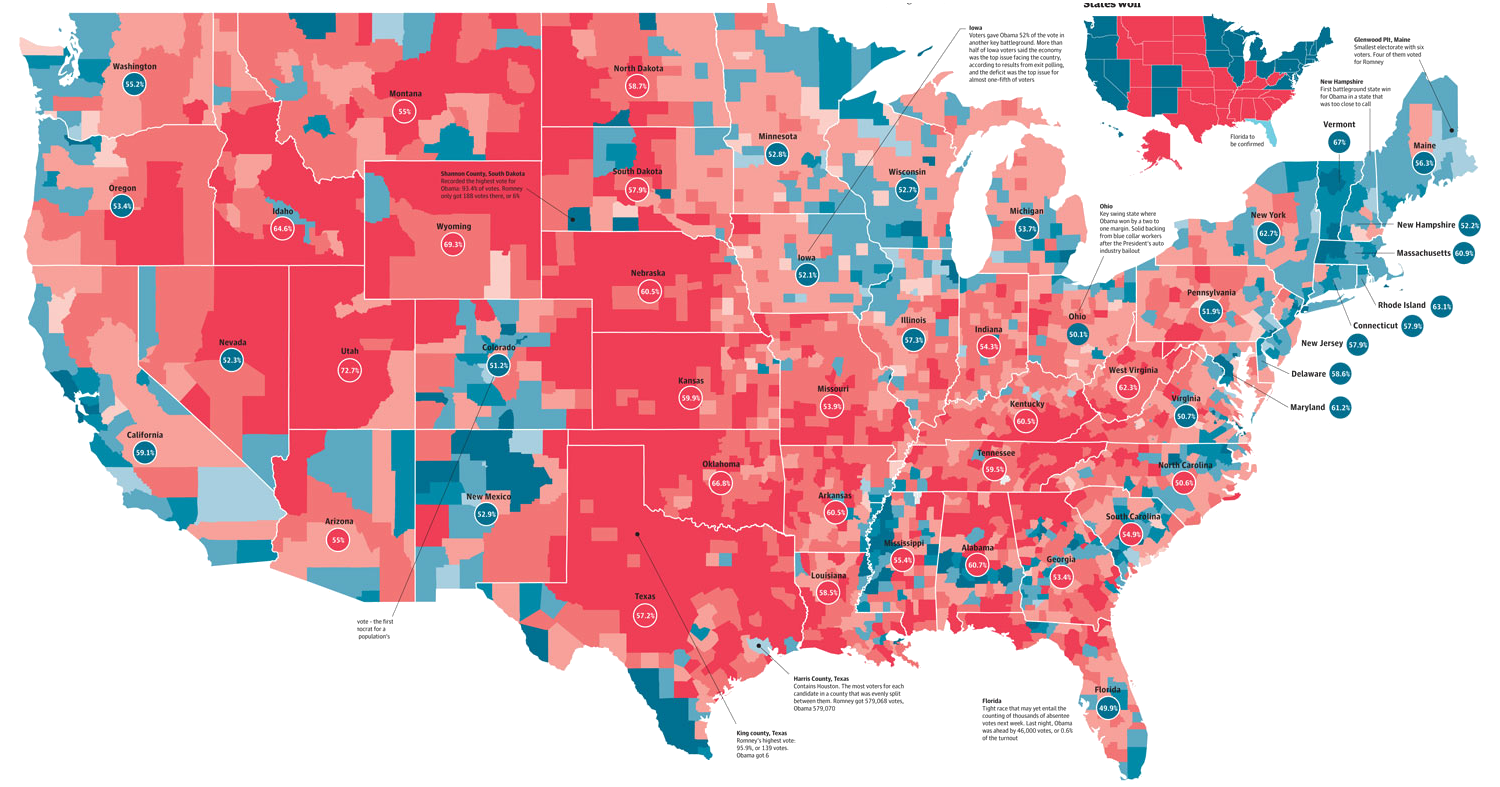
\includegraphics[width = \textwidth]{../fig/plot-binary.png} \\
\small \textbf{Divergent colour scale}\\ US presidential election 2012.\\Proportion of people voting for Democrats vs. Republicans.\\\scriptsize\emph{\cite{GuardianGraphics2012}.}
\end{figure}

\end{frame}

\section{Ternary Compositions on a Surface} %%%%%%%%%%%%%%%%%%%%%%%%%%%%%%%%%%%

\begin{frame}
\frametitle{\insertsection}

\begin{columns}[c]

\column{0.57\textwidth}
\begin{figure}[htb!]
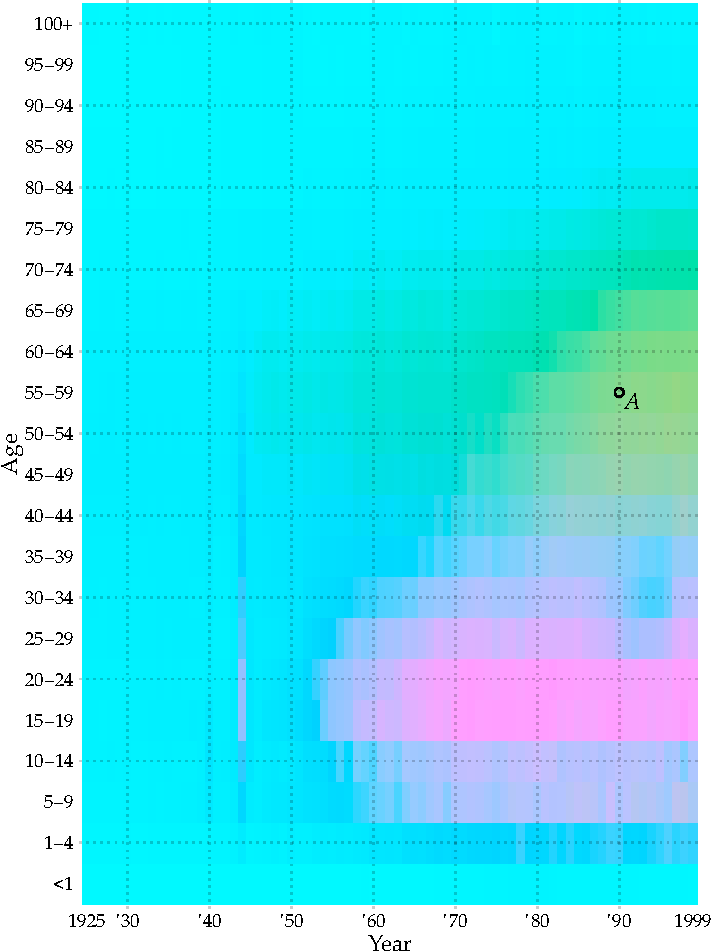
\includegraphics[width = 0.97\textwidth]{../fig/plot-tern_balance_no_lgnd.pdf}
\end{figure}

\column{0.37\textwidth}
\small \textbf{Ternary-balance-scheme}\\ Proportion of people dying from a given cause by time and age. \scriptsize\emph{France, total population.}

\begin{figure}[htb!]
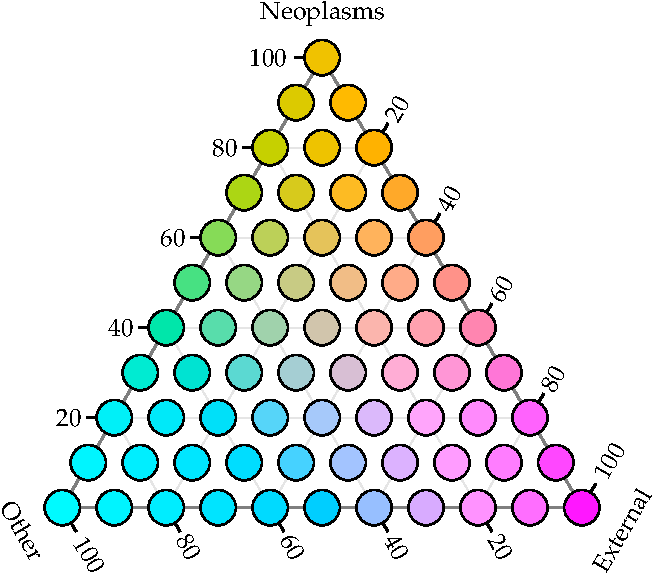
\includegraphics[width = \textwidth]{../fig/plot-tern_balance_lgnd.pdf}
\end{figure}

\end{columns}

\end{frame}

\section{N-dimensional compositions on a surface} %%%%%%%%%%%%%%%%%%%%%%%%%%%%%

\subsection{Qualitative Sequential Scheme}

\begin{frame}
\frametitle{\insertsection}

\begin{columns}[c]

\column{0.7\textwidth}
\begin{figure}[htb!]
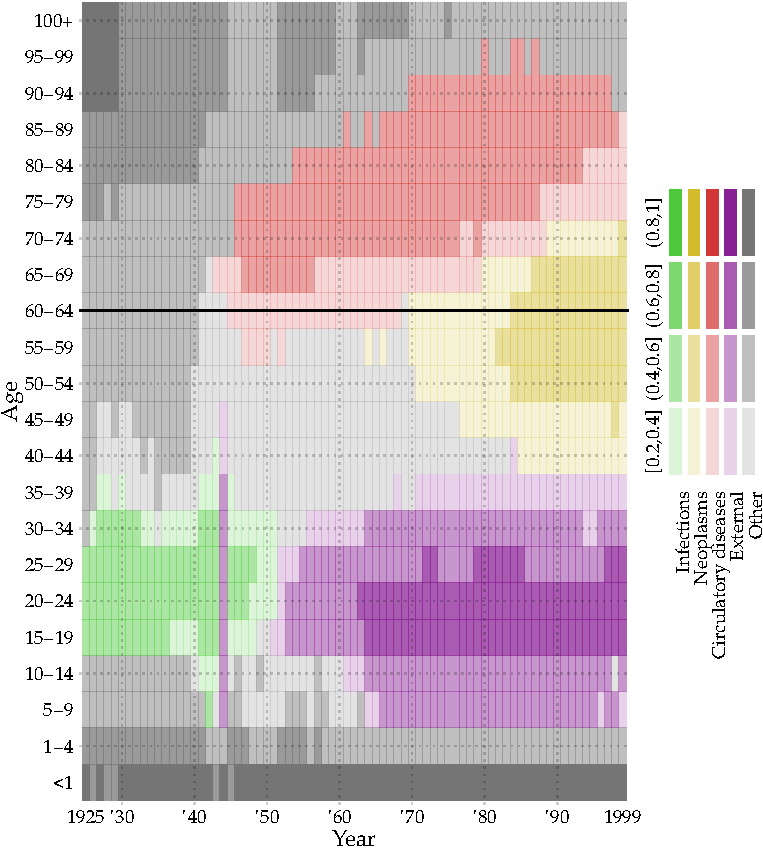
\includegraphics[width = 0.97\textwidth]{../fig/plot-qual_seq.pdf}
\end{figure}

\column{0.3\textwidth}
\footnotesize \textbf{Qualitative sequential scheme}\\ Proportion of people dying from the most prominent cause in a given time and age. \scriptsize\emph{France, total population.}

\end{columns}

\end{frame}

\section{Interlude: Brewers Typology of Colour Schemes} %%%%%%%%%%%%%%%%%%%%%%%

\begin{frame}
\frametitle{\insertsection}

\begin{columns}[c]

\column{0.75\textwidth}
\begin{figure}[htb!]
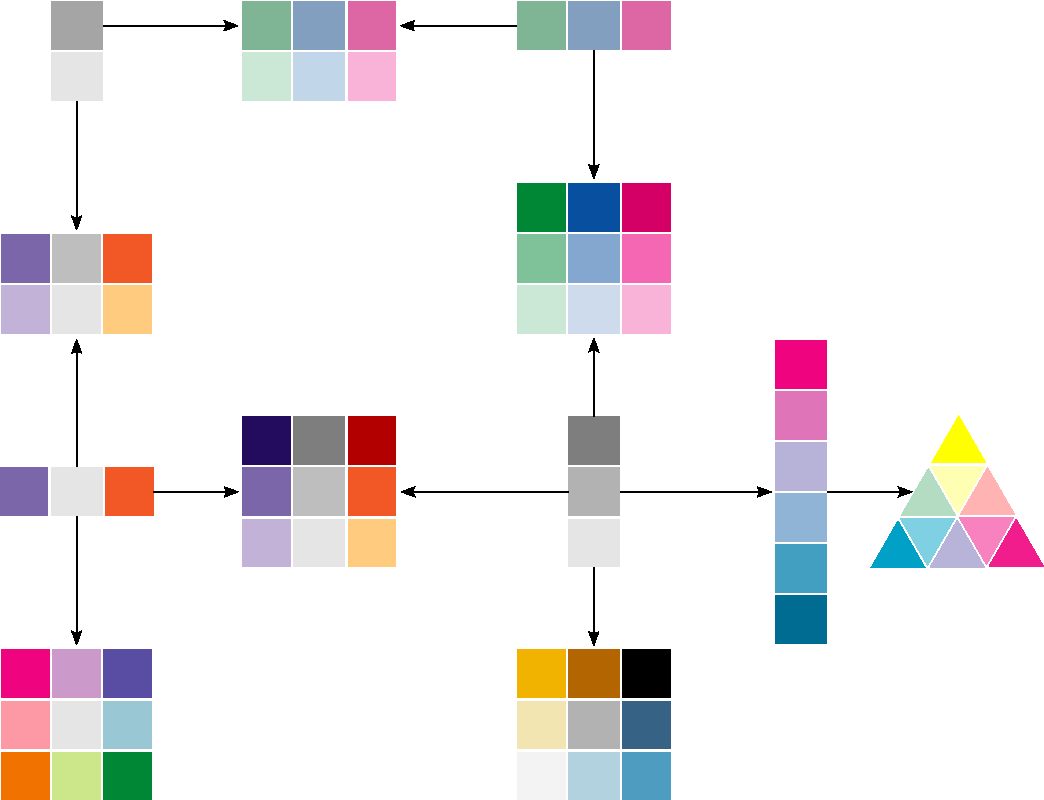
\includegraphics[width = \textwidth]{../fig/brewer_typology.pdf}\\
\end{figure}

\column{0.25\textwidth}
\footnotesize\textbf{Colour scheme typology}\\ Basic colour schemes and combinations of them. \scriptsize\emph{Redrawn from \textcite{Brewer1994}.}

\end{columns}

\end{frame}

\section{Cont'd: N-dimensional Compositions on a Surface} %%%%%%%%%%%%%%%%%%%%%

\subsection{Age-wise Area Chart}

\begin{frame}
\frametitle{\insertsection}

\begin{columns}[c]

\column{0.7\textwidth}
\begin{figure}[htb!]
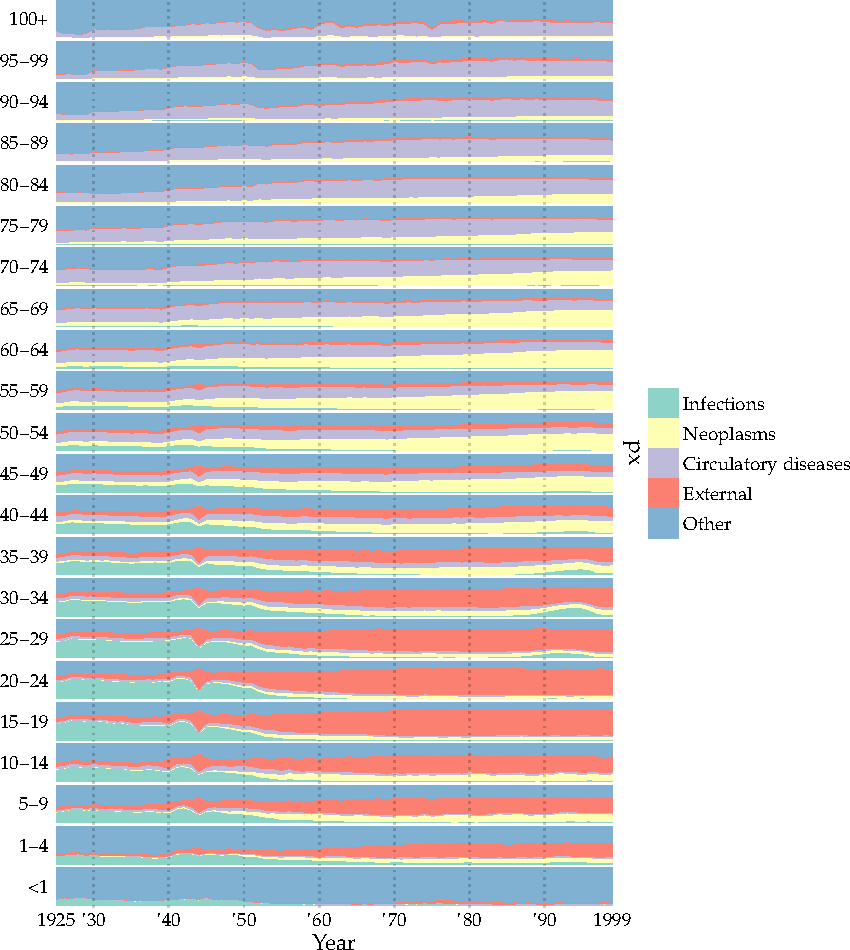
\includegraphics[width = 0.93\textwidth]{../fig/plot-agewise_area.pdf}
\end{figure}

\column{0.3\textwidth}
\small \textbf{Age-wise-area-chart}\\ Proportion of people dying from a given cause by time and age. \scriptsize\emph{France, total population.}

\end{columns}

\end{frame}

%

\subsection{Small Multiples}

\begin{frame}
\frametitle{\insertsection}

\begin{figure}[htb!]
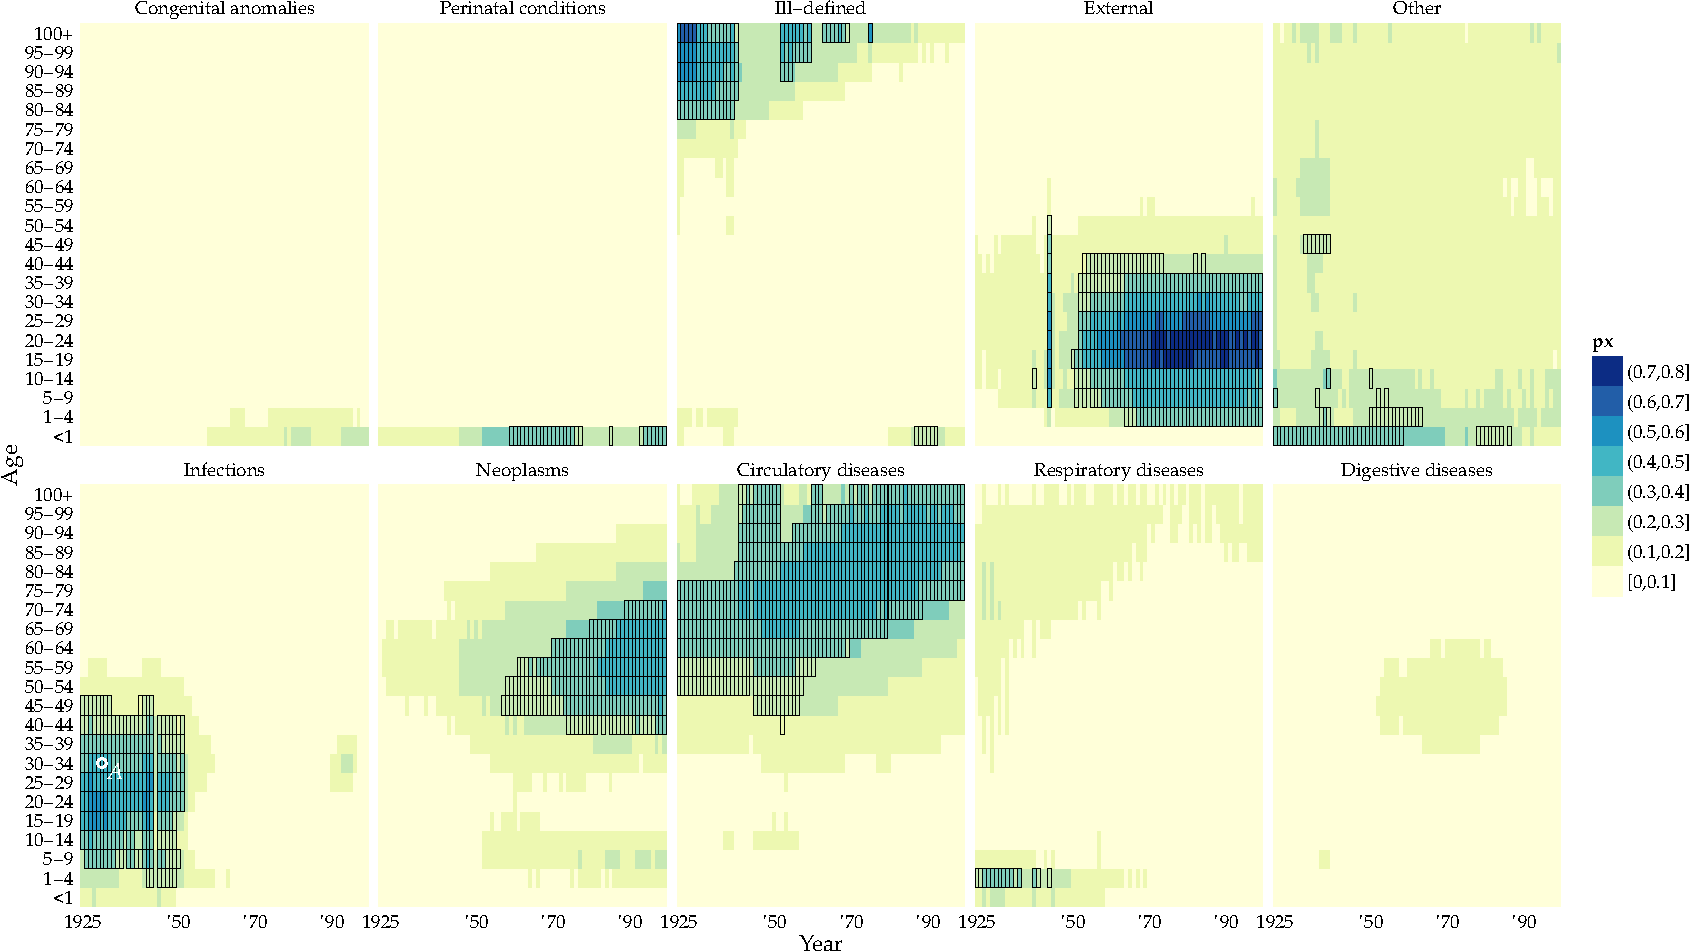
\includegraphics[width = \textwidth]{../fig/plot-small_multiples.pdf}\\
\scriptsize \textbf{Small-multiples}\\ Proportion of people dying from a given cause by time and age. \tiny\emph{France, total population.}
\end{figure}

\end{frame}

\section{References} %%%%%%%%%%%%%%%%%%%%%%%%%%%%%%%%%%%%%%%%%%%%%%%%%%%%%%%%%%

\begin{frame}
\frametitle{\insertsection}

\begin{centering}

\Large\fullcite{Schoeley2015}

\smallskip

\Large\texttt{https://github.com/jschoeley/viscomplexis}

\end{centering}

\end{frame}

%

\begin{frame}
\frametitle{\insertsection}

\nocite{MOLAST2000}

\printbibliography

\end{frame}

\end{document}